
MIKTEX
pdflatex -aux-directory=build main.tex

\todo{Plan my thesis structure before writing}

``\ldots''

\grule{}

\marginpar{Test Hello}

http://www.khirevich.com/latex/microtype/

\reflectbox{<stuff>}

\reflectbox{G}

\usepackage{CJKutf8}

\begin{CJK}{UTF8}{min}
\section{これは最初のセクションである}
日本語で \LaTeX{} の組版を実証するための導入部分。

フォントはまた、数学的な形態および他の環境で使用することができる
\end{CJK}

\begin{align}
a + b = 1, \notag \\
a + c = 42, \notag \\
a + d = 666. \label{all}
\end{align}

% break an equation and to align it in columns, just as if the parts of the equation were in a table
\begin{equation} \label{eq1}
\begin{split}
A & = \frac{\pi r^2}{2} \\
 & = \frac{1}{2} \pi r^2
\end{split}
\end{equation}

% use * to toggle the equation numbering
% first part will be aligned to the left and the second part will be displayed in the next line and aligned to the right
\begin{multline*}
p(x) = 3x^6 + 14x^5y + 590x^4y^2 + 19x^3y^3\\
- 12x^2y^4 - 12xy^5 + 2y^6 - a^3b^3
\end{multline*}

% align vertically
\begin{align*}
2x - 5y &=  8 \\
3x + 9y &=  -12
\end{align*}

% a set of consecutive equations, centered and with no alignment
\begin{gather*}
2x - 5y =  8 \\
3x^2 + 9y =  3a + c
\end{gather*}

TEST:\\
Here’s my \gls{hyper} term. \gls{holo} \gls{hyper}\\
First use: \gls{ir}. Second use: \gls{ir}.\\
First use: \gls{nlp}. Second use: \gls{nlp}.

\begin{align}
\vec{d_j} = \left(w_{1,j}, w_{2,j}, \ldots, w_{t,j} \right) \\
\vec{q} = \left(w_{1,q}, w_{2,q}, \ldots, w_{t,q} \right)
\end{align}

% COLOUR
\textcolor{red}{300 words\ldots}

\begin{comment}
\end{comment}

\begin{draft}
\end{draft}

% Use this inside {comment} or {draft} tags
\begin{shaded}
\end{shaded}

% TABLES

\begin{table}[h]
  \everyrow{\hrule}
  \tabulinesep{2mm}
  \begin{tabu}{|X|X|X|X|}


\begin{table}[!htb] % (here, top, bottom, page)
\centering
\begin{tabular}{|l|l|l|}
\hline
\textbf{Humour} & \textbf{Discovery} & \textbf{Art} \\ \hline
Laugh           & Understand         & Marvel       \\ \hline
Riddle          & Problem            & Allusion     \\ \hline
Debunking       & Discovering        & Revealing    \\ \hline
Coincidence     & Trigger            & Fate         \\ \hline
Aggressive      & Neutral            & Sympathetic  \\ \hline
\end{tabular}
\caption[Text for Table of Contents]{Caption text under table}
\end{table}

\begin{table}[h]
    \begin{subtable}[h]{0.45\textwidth}
        \centering
        \begin{tabular}{l | l | l}
        Day & Max Temp & Min Temp \\
        \hline \hline
        Mon & 20 & 13\\
        Tue & 22 & 14\\
        Wed & 23 & 12\\
        Thurs & 25 & 13\\
        Fri & 18 & 7\\
        Sat & 15 & 13\\
        Sun & 20 & 13
        \end{tabular}
        \caption{First Week}
\label{tab:week1}
    \end{subtable}
    \hfill
    \begin{subtable}[h]{0.45\textwidth}
        \centering
        \begin{tabular}{l | l | l}
        Day & Max Temp & Min Temp \\
        \hline \hline
        Mon & 17 & 11\\
        Tue & 16 & 10\\
        Wed & 14 & 8\\
        Thurs & 12 & 5\\
        Fri & 15 & 7\\
        Sat & 16 & 12\\
        Sun & 15 & 9
        \end{tabular}
        \caption{Second Week}
\label{tab:week2}
    \end{subtable}
    \caption{Max and min temps recorded in the first two weeks of July}
\label{tab:temps}
\end{table}

% FIGURES
\begin{figure}[!htb] % (here, top, bottom, page)
\centering % width=\linewidth
\includegraphics[height=0.3\textheight]{images/Electron.png}
\caption[Text for Table of Contents]{Caption text under figure}
\label{fig:Electron}
\end{figure}

% CITATIONS
\citet{jon90}	               -->    	Jones et al. (1990)
\citet[chap. 2]{jon90}	     -->    	Jones et al. (1990, chap. 2)
\citep{jon90}	               -->    	(Jones et al., 1990)
\citep[chap. 2]{jon90}	     -->    	(Jones et al., 1990, chap. 2)
\citep[see][]{jon90}	       -->    	(see Jones et al., 1990)
\citep[see][chap. 2]{jon90}	 -->    	(see Jones et al., 1990, chap. 2)
\citet*{jon90}	             -->    	Jones, Baker, and Williams (1990)
\citep*{jon90}	             -->    	(Jones, Baker, and Williams, 1990)



% CODE

\begin{lstlisting}
// Hello.java
import javax.swing.JApplet;
import java.awt.Graphics;

public class Hello extends JApplet {
    public void paintComponent (Graphics g) {
        g.drawString (``Hello, world!'', 65, 95);
    }
}
\end{lstlisting}

\begin{wrapfigure}{r}{0.5\textwidth}
  \begin{center}
    \includegraphics[width=0.48\textwidth]{gull}
  \end{center}
  \caption{A gull}
\end{wrapfigure}

% SUBFIGURES
\begin{figure}
\centering
\begin{minipage}{.275\linewidth}
  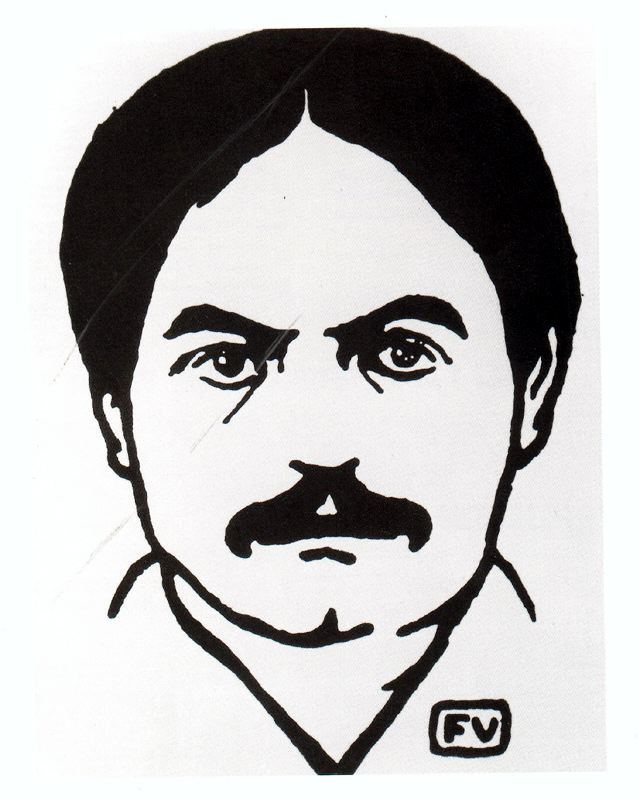
\includegraphics[width=\linewidth]{FelixVallotton}
  \caption[figure1]{FelixVallotton}
\label{img1}
\end{minipage}
\hspace{.05\linewidth}
\begin{minipage}{.275\linewidth}
  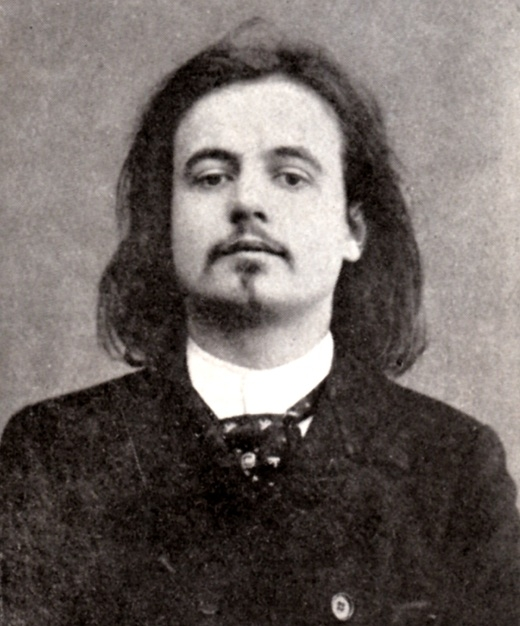
\includegraphics[width=\linewidth]{jarry}
  \caption[figure2]{jarry}
\label{img2}
\end{minipage}
\hspace{.05\linewidth}
\begin{minipage}{.275\linewidth}
  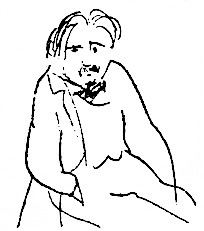
\includegraphics[width=\linewidth]{jpicasso}
  \caption[figure3]{jpicasso}
\label{img3}
\end{minipage}
\end{figure}


% CODE

\lstset{ %
  backgroundcolor=\color{white},   % choose the background color; you must add \usepackage{color} or \usepackage{xcolor}
  basicstyle=\footnotesize,        % the size of the fonts that are used for the code
  breakatwhitespace=false,         % sets if automatic breaks should only happen at whitespace
  breaklines=true,                 % sets automatic line breaking
  captionpos=b,                    % sets the caption-position to bottom
  commentstyle=\color{mygreen},    % comment style
  deletekeywords={\ldots},            % if you want to delete keywords from the given language
  escapeinside={\%*}{*)},          % if you want to add LaTeX within your code
  extendedchars=true,              % lets you use non-ASCII characters; for 8-bits encodings only, does not work with UTF-8
  frame=single,                    % adds a frame around the code
  keepspaces=true,                 % keeps spaces in text, useful for keeping indentation of code (possibly needs columns=flexible)
  keywordstyle=\color{blue},       % keyword style
  language=Octave,                 % the language of the code
  otherkeywords={*,\ldots},            % if you want to add more keywords to the set
  numbers=left,                    % where to put the line-numbers; possible values are (none, left, right)
  numbersep=5pt,                   % how far the line-numbers are from the code
  numberstyle=\tiny\color{mygray}, % the style that is used for the line-numbers
  rulecolor=\color{black},         % if not set, the frame-color may be changed on line-breaks within not-black text (e.g. comments (green here))
  showspaces=false,                % show spaces everywhere adding particular underscores; it overrides 'showstringspaces'
  showstringspaces=false,          % underline spaces within strings only
  showtabs=false,                  % show tabs within strings adding particular underscores
  stepnumber=2,                    % the step between two line-numbers. If it's 1, each line will be numbered
  stringstyle=\color{mymauve},     % string literal style
  tabsize=2,                       % sets default tabsize to 2 spaces
  title=\lstname{}                   % show the filename of files included with \lstinputlisting; also try caption instead of title
}
